\begin{table*}
  \centering
  \small
  \begin{tabular}{llcccccccac@{}}
    \toprule
    \multirow{4}{*}{\vspace{0em}\textbf{Model}} 
    & \phantom{} 
    & \multicolumn{2}{c}{\textbf{Modality}} 
    & \phantom{}
    & \multicolumn{4}{c}{\textbf{Reasoning Type}} 
    & \cellcolor{white}
    & \phantom{}\\
    
    \cmidrule{3-4} \cmidrule{6-9} 

    \phantom{} 
    & \phantom{} 
    & \textbf{Table} 
    & \textbf{Figure}   
    & \phantom{}  
    & \textbf{COM} 
    & \textbf{DE} 
    & \textbf{LOC} 
    & \textbf{VU} 
    & \textbf{All} \\

\midrule
Expert Performance & & 0.678 & 0.765 & & 0.751 & 0.872 & 0.711 & 0.732 & 0.796\\
Random & & 0.134 & 0.106 & & 0.134 & 0.130 & 0.110 & 0.111 & 0.126 \\
\midrule
\multicolumn{11}{c}{\textbf{Simple Baselines}}  \\ 
\midrule
\texttt{text-embedding-3-large} & & 0.321 & 0.239 & & 0.267 & 0.323 & 0.384 & 0.218 & 0.297\\
%
\texttt{text-embedding-3-small} & & 0.223 & 0.205 & & 0.221 & 0.223 & 0.267 & 0.138 & 0.217\\
%
\texttt{text-embedding-ada-002} & & 0.185 & 0.168 & & 0.200 & 0.171 & 0.224 & 0.096 & 0.180\\
%
Contriever & & 0.165 & 0.229 & & 0.196 & 0.144 & 0.274 & 0.142 & 0.184\\
%
BM25 & & 0.138 & 0.098 & & 0.118 & 0.128 & 0.160 & 0.110 & 0.127\\
%
\midrule
\multicolumn{11}{c}{\textbf{Open-Source Large Multi-modal Models (LMMs)}} \\ 
\midrule

InternVL-Chat-V1.1 & & 0.168 & 0.084 & & 0.136 & 0.153 & 0.170 & 0.109 & 0.144\\
Yi-VL-34B & & 0.105 & 0.057 & & 0.101 & 0.088 & 0.080 & 0.086 & 0.091\\
Qwen-VL-Plus & & 0.065 & 0.131 & & 0.077& 0.053 & 0.148 & 0.136 & 0.089\\
LLaVA-1.6 & & 0.079 & 0.000 & & 0.088 & 0.044 & 0.052 & 0.000 & 0.056\\
DeepSeek-VL & & 0.075 & 0.087 & & 0.064 & 0.081 & 0.109 & 0.070 & 0.079\\
%
% \addlinespace[0.2em]\hdashline\addlinespace[0.2em]
\midrule
\multicolumn{11}{c}{\textbf{Proprietary Large Multi-modal Models (LMMs)}} \\ 
\midrule
%
GPT-4o & & \bb{0.520} & \bb{0.454} & & \bb{0.443} & \bb{0.565} & \bb{0.570} & \underline{0.418} & \bb{0.500}\\
%
GPT-4V(ision) & & \underline{0.440} & 0.309 & & \underline{0.383} & \underline{0.407} & \underline{0.523} & 0.288  & \underline{0.400}\\
%
Claude-3-Sonnet & & 0.385 & \underline{0.369} & & 0.357 & 0.363 & 0.395 & \bb{0.422} & 0.374\\
%
Claude-3-Opus & & 0.256 & 0.343 & & 0.320 & 0.362 & 0.301 & 0.204 & 0.316\\
%
Gemini-Pro-Vision-1.0 & & 0.217 & 0.188 & & 0.196 & 0.160 & 0.284 & 0.195 & 0.197\\
%
Claude-3-Haiku & & 0.189 & 0.188 & & 0.194 & 0.201 & 0.130 & 0.208 & 0.188\\
\bottomrule
\end{tabular}
\caption{
Mean reciprocal rank (MRR) on the \emph{test} set of \data. The best-performing model in each category is \textbf{bold}, and the second best is {\underline{underlined}}. Reasoning types: \textbf{COM}: comparison, \textbf{DE}: data extraction, \textbf{LOC}: location, \textbf{VU}: visual understanding.
}
\label{tab:locality_mrr}

\end{table*}
\begin{table*}[!t]
\centering
\small
\begin{tabular}{@{}lrcccccac@{}}
\toprule
\textbf{Model} 
& \textbf{\begin{tabular}[c]{@{}c@{}}Context \\Window\end{tabular}}
& \textbf{\begin{tabular}[c]{@{}c@{}}CU\end{tabular}} 
& \textbf{\begin{tabular}[c]{@{}c@{}}II\end{tabular}} 
& \textbf{\begin{tabular}[c]{@{}c@{}}RDI\end{tabular}} 
& \textbf{\begin{tabular}[c]{@{}c@{}}MA\end{tabular}} 
& \textbf{\begin{tabular}[c]{@{}c@{}}CA\end{tabular}} 
& \textbf{\begin{tabular}[c]{@{}c@{}}All\end{tabular}} 
\\ \midrule

Expert Performance &  & 72.32 & 71.11 & 83.15 & 76.84 & 79.17 & 76.50\\ 

\midrule
\multicolumn{8}{c}{\textbf{Open-Source Large Language Models (LLMs)}} \\ 
\midrule
%
$^\dagger$Command R+ & 128,000  & \bb{40.00} & 22.73 & \bb{33.33} & \bb{37.91} & \bb{39.53} & \bb{33.25}\\
%
Llama-3-70B & 8192 & \underline{31.35} & \bb{35.23} & 22.84 & 32.49 & 35.19 & \underline{31.30} \\
%
Mistral-7B & 32,768  & 17.10 & 24.09 & 8.89 & 25.81 & 26.72 & 20.45\\
%
PaLM-2 & 36,864 & 20.73 & 26.42 & 16.35 & 27.65 & 26.72  & 23.55\\
%
DBRX & 32,768  & 18.13 & 19.43 & 13.94 & 21.30 & 22.63 & 19.05 \\
%
Gemma-7B & 8,192 & 8.89 & 15.15 & 1.39 & 13.95 & 20.93  & 12.25 \\
%
\midrule
\multicolumn{8}{c}{\textbf{Proprietary Large Language Models (LLMs)}} \\ 
\midrule
%
$^\dagger$GPT-3.5 & 16,385 & 22.22 & \underline{33.33} & 19.44 & \underline{32.56} & \underline{37.21} & 29.00 \\
%
$^\dagger$GPT-4 & 128,000 & 31.11 & 21.21 & \underline{23.61} & \underline{32.56} & 31.40 & 28.50 \\
%
$^\dagger$Claude-3-Haiku & 200,000 & 28.89 & 30.88 & 12.50 & 29.07 & 38.10  & 28.25  \\ 
%
$^\dagger$Claude-3-Sonnet & 200,000 & 25.56 & 21.21 & 19.44 & 25.58 & 38.37 & 26.50 \\
%
$^\dagger$Claude-3-Opus  & 200,000 & 26.67 & 18.18 & 20.83 & 26.74 & 30.23 & 25.00\\
%
$^\dagger$Gemini-Pro-1.0 & 30,720 & 18.89 & 19.70 & 18.06 & 22.09 & 29.07  & 21.75\\
%
\bottomrule
\end{tabular}
%

\caption{
LLM-based accuracy score on the \emph{test} set of \data in \emph{retrieval} setting from GPT-4o's ranking. The best-performing model in each category is \textbf{bold}, and the second best is {\underline{underlined}}. Human expert performance is assessed in an oracle setting, where the correct reference paper is pre-identified. Reasoning types: \textbf{CU}: conceptual understanding, \textbf{II}: implications and Inferences, \textbf{RDI}: results and data interpretation, \textbf{MA}: methodological analysis, \textbf{CA}: critical analysis. $^\dagger$: Due to budget constraints, we randomly sampled 200 instances from the \emph{test} set for evaluation.
}
\label{tab:detail_gpt_based}
\end{table*}





\section{Experiments}

We evaluate 18 foundation models, including both \emph{open-source} and \emph{proprietary} LMMs and LLMs. 
%
For each model, we select the most recent, largest, and best-performing checkpoint as of April 15th, 2024. 
%
The evaluation of the \data benchmark is structured into two distinct stages: \emph{visual context} evaluation and \emph{reference-based} evaluation.


\subsection{Visual Context Evaluation}

\paragraph{Task Formulation.}
The visual context evaluation with LMMs is defined as follows: 
%
Given a visual context question $Q_{vis}$, its correspondent scientific image $I$, and a list of reference papers $D = \{d_1, d_2, \cdots, d_n\}$, the objective is to determine a ranking of these papers based on their relevance to the question and the image. 
%
This ranking is represented by $R = \{r_1, r_2, \cdots, r_n\}$, where $r_i$ denotes the ranking of the paper $d_i$ for each index $i \in \{1, 2, \cdots, n\}$.
%
We input $Q_{vis}$, $I$ and $D$ into each LMM, denoted by $f_{LMM}$, and instruct it to generate a ranking $R$ of $D$ based on their relevance to $Q_{vis}$ and $I$:
\begin{equation*}
    R = f_{LMM}(Q_{vis}, I, d_1, d_2, \cdots, d_n)
\end{equation*}
For comparative analysis, simple baselines presented in Table \ref{tab:locality_mrr} are also assessed for the ranking task. 
%
Other than BM25, these baselines employ cosine similarity between query and document embeddings to rank documents. 
%
Each query combines the visual context question $Q_{vis}$ and its image caption $C$ generated by GPT-4o with one of the documents, represented by its title and abstract. 
%
Given a visual context question $Q_{vis}$, its correspondent scientific image $I$, a list of reference papers $D = \{d_1, d_2, \cdots, d_n\}$, an embedding model $\textit{Embed}$, and a cosine similarity function $\textit{sim}$, the ranking process is defined as below:
\begin{equation*}
    \begin{aligned}
        &C = \textit{GPT-4o}(I)\\
        &q = \textit{Embed}(\textit{concat}(Q_{vis}, C))\\
        &\forall d_i \in D, h_i = \textit{Embed}(d_i)\\
        &R = \textit{sort}(sim(q, h_1), \cdots, sim(q, h_n))
    \end{aligned}
\end{equation*}




\paragraph{Evaluation Protocol.}

At the visual context evaluation stage, we assess LMMs' ability to accurately retrieve and rank the correct reference paper from a complete list of reference papers. 
%
Performance is measured using an established information retrieval metric, Mean Reciprocal Rank (MRR), which effectively gauges a model's ability to identify and prioritize the most relevant reference paper. 
%
We also calculate Recall@k and nDCG@k to further analyze LMMs' retrieval effectiveness, with results detailed in Table \ref{tab:recall@k} and \ref{tab:ndcg@k} in Appendix \ref{more_result_analysis}.



\paragraph{Experiment Setup.}
This stage involves five \emph{open-source} LMMs, including \emph{open-source} models, such as 
LLaVA 1.6 \cite{liu2023visual}, 
InternVL-Chat-1.1V \cite{chen2024internvl}, 
Yi-VL-34B \citep{ai2024yi},
DeepSeek-VL \citep{deepseekvl},
and Qwen-VL-Plus \cite{bai2023qwenvl}; 
six \emph{proprietary} LMMs, including 
GPT-4V(ision) \cite{openai2024gpt4},
GPT-4o \cite{gpt-4o}, 
Claude 3 Haiku \citep{claude3},
Claude 3 Sonnet \citep{claude3},
Claude 3 Opus \citep{claude3},
and Gemini Vision Pro 1.0 \cite{geminiteam2023gemini}; 
and five \emph{simple baselines}, including 
BM25, 
Contriever \cite{izacard2021contriever}, 
and OpenAI Embeddings\footnote{\url{https://platform.openai.com/docs/guides/embeddings}} (\texttt{Large}, \texttt{Small}, and \texttt{Ada}).



\subsection{Reference-Based Evaluation}

\paragraph{Task Formulation.}
The reference-based evaluation is defined as follows:
Given a combined question $Q_{comb}$ and a ranking $R$ of the reference papers obtained in the \emph{visual context} evaluation stage, the objective is to answer the question based on the top $k$ ranked paper in $R$, denoted by $\textit{Top}_k(R) = \{R[1], R[2], \cdots, R[k]\}$. 
%
Since \emph{combined} questions contain elements from both \emph{visual context} and \emph{reference-based} questions, we instruct LLMs to solely concentrate on the \emph{reference-based} aspect of $Q_{comb}$. 
%
The prompts used for this instruction are detailed in Table \ref{tab:detail prompt} in Appendix \ref{appx:prompt_for_combined_questions}.
%
Accordingly, we input $Q_{comb}$ and $\textit{Top}_k(R)$ into LLMs, denoted by $f_{LLM}$, and instruct LLMs to answer $Q_{comb}$ based on the textual content in top $k$ ranked papers: 
\begin{equation*}
    \textit{Ans} = f_{LLM}(Q_{comb}, R[1], R[2], \cdots, R[k])
\end{equation*}


\paragraph{Evaluation Protocol.}

At the reference-based evaluation stage, we assesses how LLMs perform on reference-based questions using the top three ranked papers identified from the visual context evaluation stage as context. 
%
Specifically, these papers are ranked by GPT-4o, which is highlighted as the most effective retrieval model in Table \ref{tab:locality_mrr}. GPT-4o achieves an MRR of 0.488, suggesting that the correct reference paper typically appears in the 2.1-th position, placing it within the top three ranked papers on average.
%
Given that both reference-based question and answer generation utilize plain text extracted from TeX files, we employ the same parsed TeX files as input for LLMs to solve the text-only, reference-based questions. 


\paragraph{Generative Response Metrics.}

Following effectiveness of LLMs in evaluating the quality of short AI-generated responses \cite{wang2023evaluating, lu2024mathvista, alpacafarm, charxiv}, we utilize a strong LLM-evaluator (GPT-4) to evaluate the quality of responses generated in the reference-based evaluation stage.
%
Specifically, the LLM-evaluator rates answers generated against the \emph{gold answers} using a scoring scale of 0, 0.5, and 1.
%
To more closely align our scoring scale with expert assessments, we compute \emph{Cohen's Kappa} \cite{cohen's_kappa} to assess the agreement between the LLM-evaluator and expert annotators. 
%
This comparison is conducted for both the 0-0.5-1 and the 1-2-3-4-5 scales, with prompts utilized for evaluation provided in Table \ref{tab:gpt_based_evaluator_app} in Appendix~\ref{cohen's kappa}. 
%
Expert annotators are tasked with rating 200 responses from four different LLMs (Command R+, GPT-4, Mistral, and Gemma) using both scales. 
%
Our calculations reveal a Cohen's Kappa value of 0.520 for the 0-0.5-1 scale and 0.444 for the 1-2-3-4-5 scale. 
%
These results demonstrate greater consistency with expert evaluations when using the 0-0.5-1 scale. 
%
Further details and comparative results are presented in Appendix~\ref{cohen's kappa}.
%
Thus, we adopt the 0-0.5-1 scoring scale for our evaluations.
%
Additionally, we employ established metrics such as ROUGE \cite{lin-2004-rouge}, BERTScore \cite{zhang2020bertscore}, and AutoACU \cite{autoacu} to further gauge the quality of the generated responses.
Detailed results are provided in Table \ref{tab:ROUGE}, \ref{tab:bertscore}, \ref{tab:autoacu} in Appendix \ref{more_result_analysis}.


\paragraph{Experiment Setup.}

This stage involves six \emph{open-source} Text-Only LLMs, including
Mistral-7B \cite{jiang2023mistral}, 
Llama-3-70B \cite{llama3}, 
DBRX \cite{DBRX}, 
PaLM-2 \citep{palm2},
Gemma \citep{gemma},
and Command R+ \cite{commandR+};
and six \emph{proprietary} LLMs, including 
GPT-3.5 \citep{gpt3.5}, 
GPT-4 \cite{openai2024gpt4}, 
Claude 3 Haiku \citep{claude3}, 
Claude 3 Sonnet \citep{claude3}, 
Claude 3 Opus \cite{claude3}, 
and Gemini-Pro-1.0 \cite{geminiteam2023gemini}.



\begin{figure*}[!t]
\centering
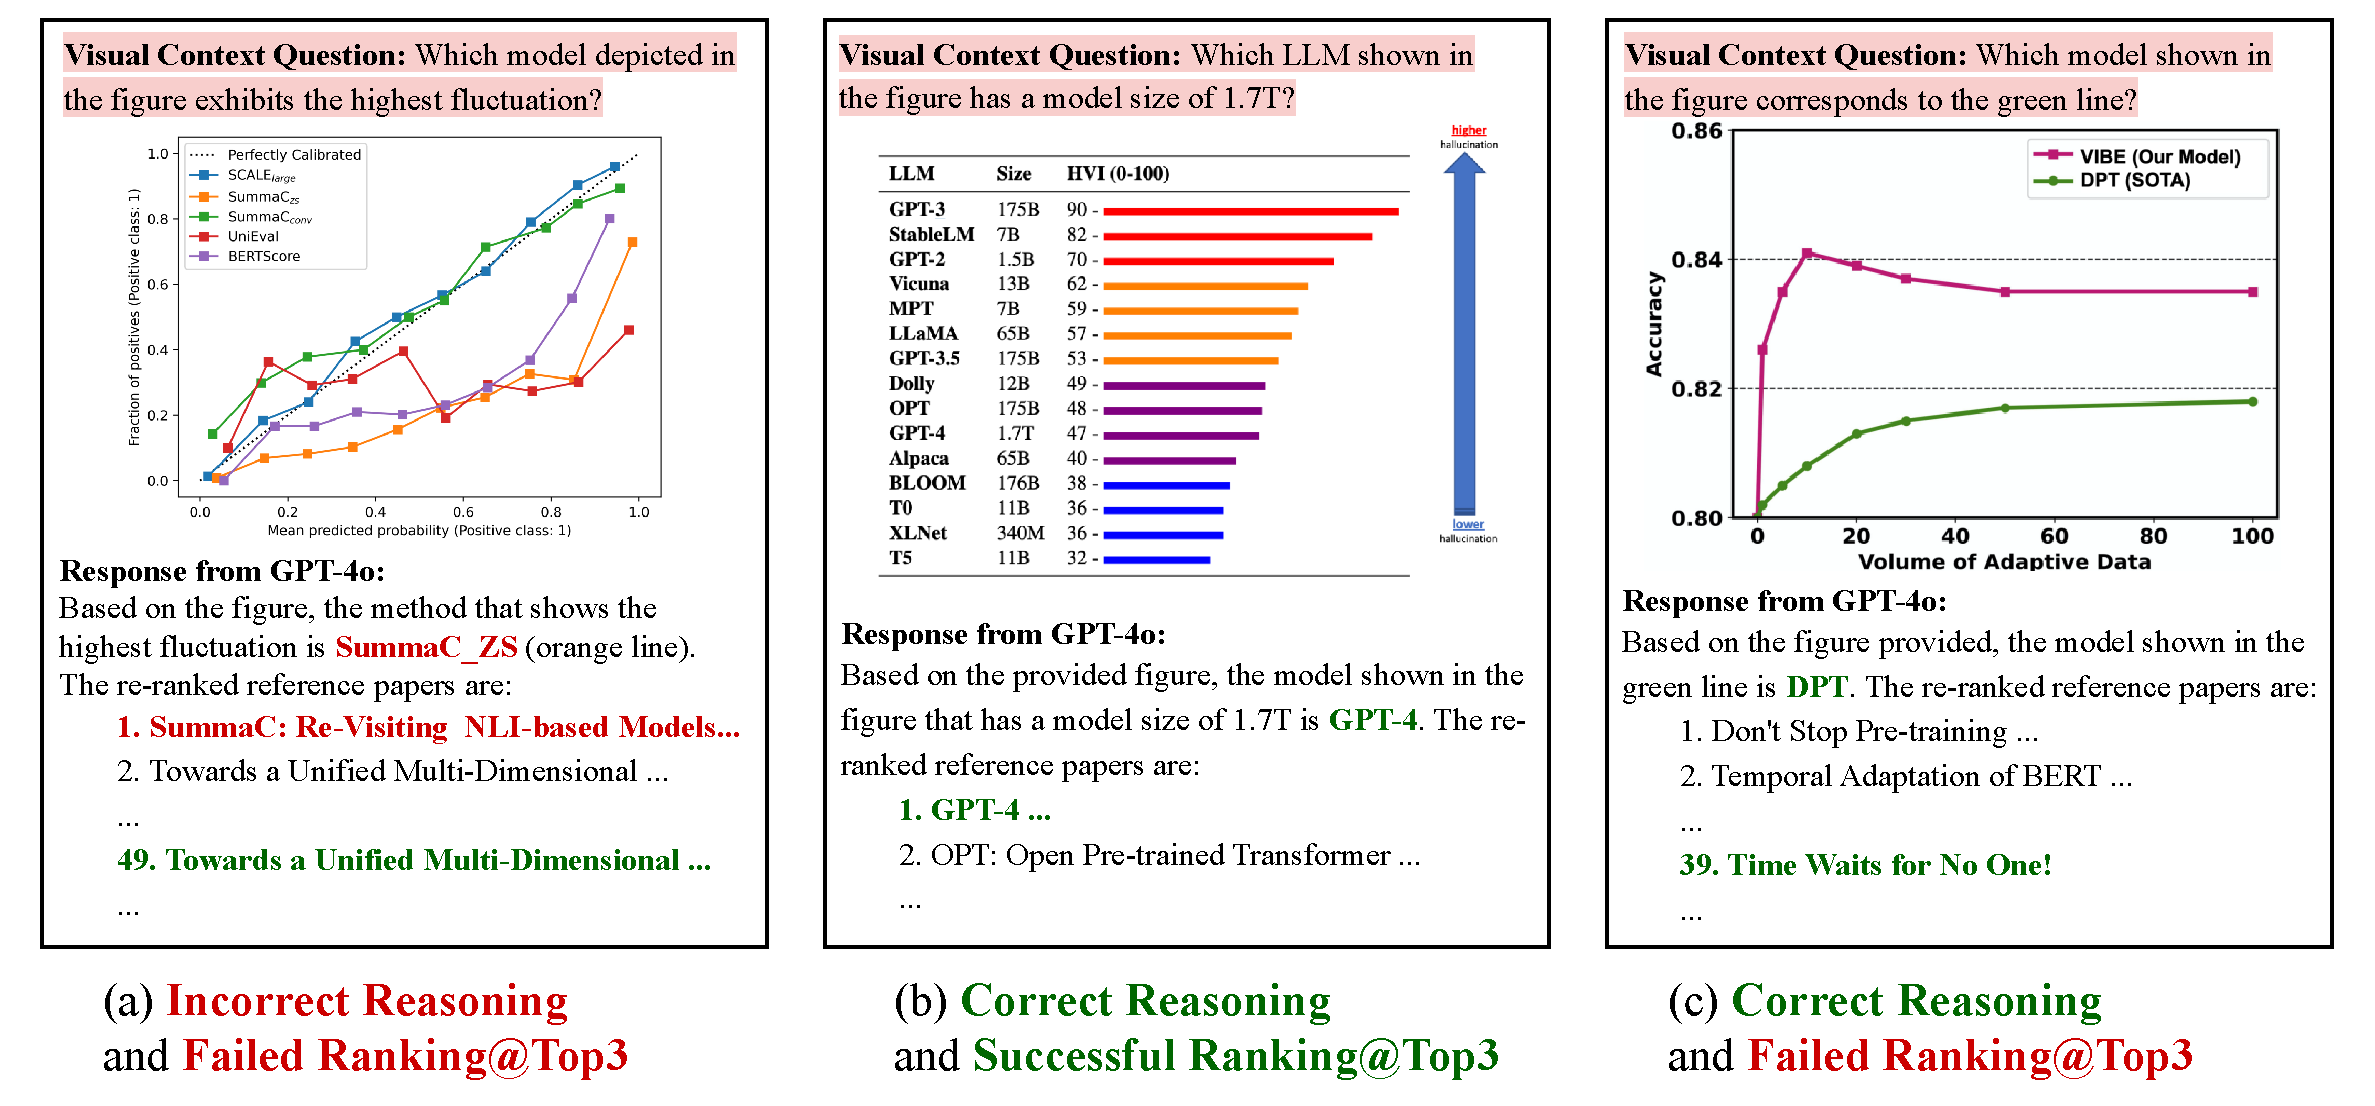
\includegraphics[width=1\textwidth]{raw_figures/visual_fine_grained.pdf}
\caption{Three examples from GPT-4o in answering visual context questions.
} 
\label{fig:fine-grained}
\end{figure*}
\subsection{Main Results}

\label{main_result}
Table \ref{tab:locality_mrr} and Table \ref{tab:detail_gpt_based} present our main results for both \emph{open-source} and \emph{proprietary} LMMs and LLMs on the validation and test set of \data, focusing on \emph{visual context} and \emph{reference-based} questions, respectively. 
%
We summarize our key findings as follows:


\paragraph{Finding 1: Challenges in Visual Reasoning and Paper Ranking with \data.}
%
Table \ref{tab:locality_error_analysis} provides a breakdown of GPT-4o's performance in answering the visual context questions, categorized by both reasoning and ranking outcomes. 
%
Despite being the overall best-performing retriever, GPT-4o still struggles with the dual challenges: it fails to correctly interpret 42.4\% of the scientific images; even when it does produce correct visual reasoning, it falls short in ranking the associated paper within the top three choices. 
%
Notably, one interesting error pattern is the scenario ``\xmark reasoning \cmark ranking@top3,'' which accounts for 19.7\% of the cases for GPT-4o. 
%
While this type of error occurs in both open-source and proprietary LMMs, it is more prevalent in the former.
%
Example error analyses are presented in Figure \ref{fig:fine-grained}, offering a more granular view of these patterns and specific instances where the model underperforms. 

\begin{table}[!t]
  \centering
  \small
  \begin{tabular}{ccc}
    \toprule
    \textbf{\begin{tabular}[c]{@{}c@{}}Reasoning \\Correctness\end{tabular}} & 
    \textbf{\begin{tabular}[c]{@{}c@{}}Ranking@Top3\end{tabular}} & 
    \textbf{\begin{tabular}[c]{@{}c@{}}Percentage\end{tabular}} \\
    \midrule
    \cmark & \cmark & 33.0\% \\
    \cmark & \xmark & 24.7\% \\
    \xmark & \cmark & 19.7\% \\
    \xmark & \xmark & 22.7\% \\
    \bottomrule
  \end{tabular}
  \caption{Performance distribution for GPT-4o on visual context questions, categorized by \bb{Reasoning Correctness} and \bb{Ranking@Top3}.}
  \label{tab:locality_error_analysis}
\end{table}




\paragraph{Finding 2: Inherent Limitations of \emph{Open-Source} LMMs in Long-Range Ranking Task.}
%
The performance of open-source LMMs in long-range ranking tasks is significantly hindered by their fundamental limitations. We identify three primary challenges:
(1) \emph{Limited Context Window}, which necessitates division of large paper clusters into smaller segments, complicating the ranking process and potentially omitting relevant reference papers;
(2) \emph{Hallucinations}, characterized by the erroneous generation and prioritization of irrelevant arXiv webpage URLs, professional NLP terms, repetitive paper IDs, and random numerical values;
(3) \emph{Formatting Issues}, where models disregard specified format and list papers in plain text, complicating the integration of results across rankings from segmented paper clusters.
These challenges significantly impede the models' ability to provide a comprehensive evaluation of their visual reasoning capabilities, suggesting the need for improvements in their basic functionality to handle more complex reasoning and ranking tasks. A detailed evaluation of open-source LMMs is presented in Appendix \ref{app:LMMs_in_locality}. 




\paragraph{Finding 3: Precision-Recall Balance.} 
We evaluate LLMs in retrieval settings using the top $k$ ranked papers from the \emph{visual context} evaluation performed by GPT-4o for the values $k \in \{1, 2, 3, 4, 5\}$. 
As shown in Figure \ref{fig:performance_score_different_k}, performance generally increases from $k = 1$ to $k = 3$, aligning with an MRR score of approximately 0.488, which places the correct reference paper in the 2.1-th position on average. Beyond this point, as more papers are considered, more noise is introduced. The general decline in performance after $k = 3$ demonstrates models' limitations in retrieval tasks when given more irrelevant information.

\begin{figure}[!hbt]
\centering
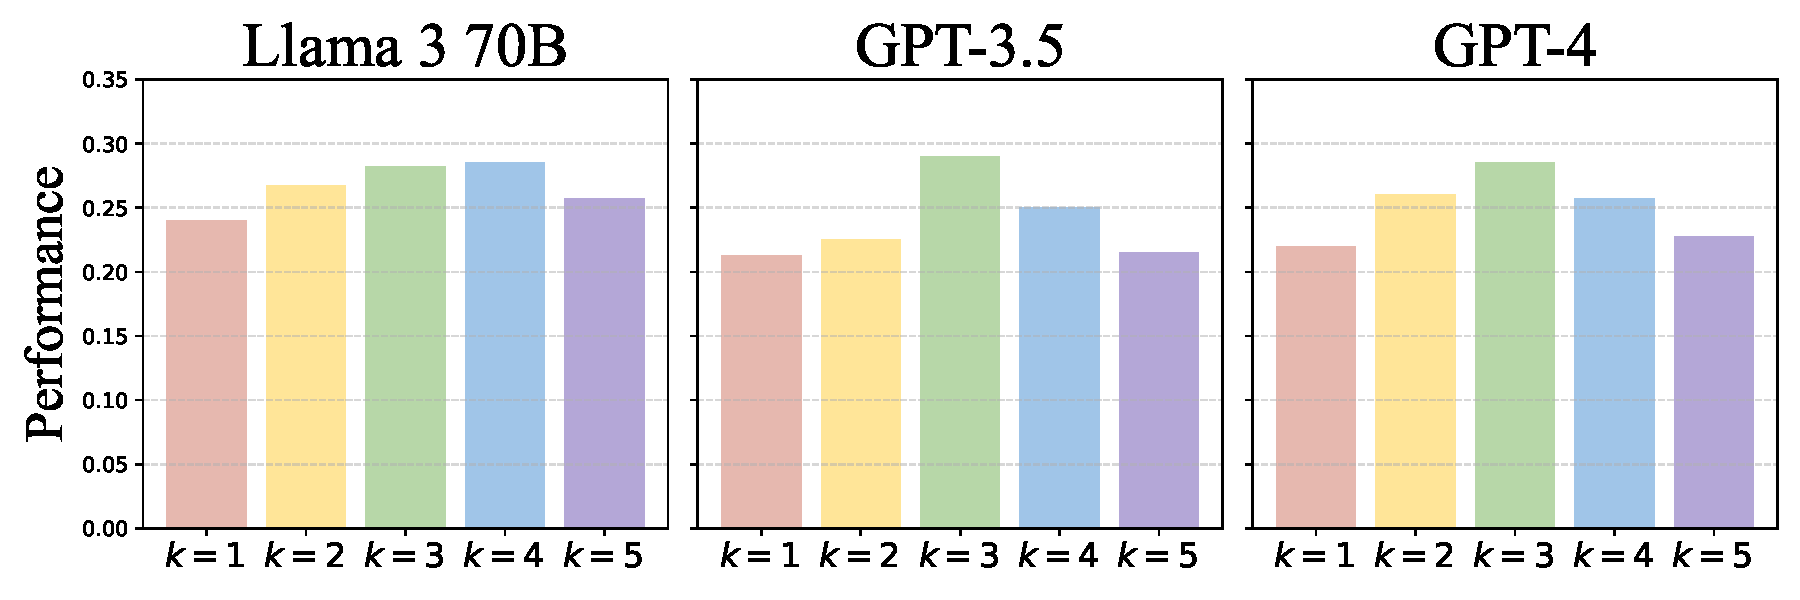
\includegraphics[width=1\linewidth]{raw_figures/Performance_Scores_Histogram.pdf}
\caption{Performance scores of Mistral, Llama 3 70B, GPT-3.5, and GPT-4 in different \emph{retrieval} settings.}


\label{fig:performance_score_different_k}
\end{figure}




\paragraph{Finding 4: Challenges in Instruction Compliance for LLMs in Retrieval Task.} 
Our evaluation of four models in both a \emph{title-only} setting, where only the title of the reference paper is provided, and a \emph{retrieval} setting, with the top three ranked papers by GPT-4o, highlights variations in instruction compliance. 
Models are instructed to answer ``I don't know'' if a definitive answer cannot be derived from the given information. 
This directive tests the models' adherence to instructions, since the task is infeasible with the titles alone and compliant models should exhibit minimal performance.
Transition to the \emph{retrieval} setting should reveal a significant increase for the models, as observed with GPT-4 in Table \ref{tab:finding4}.
Additionally, employing a LLM-based evaluator to assess generative response overlooks models' confidence levels. Less compliant models, relying on pre-trained knowledge, often produce tangentially relevant responses rather than the instructed ``I don't know,'' leading to disproportionately higher evaluations from the LLM-based evaluator.

\definecolor{deepgreen}{rgb}{0.0, 0.5, 0.0}

\begin{table}[!h]
  \centering
  \small
  \begin{tabular}{lcccc}
    \toprule
    \bb{Models} & GPT-4 & GPT-3.5 & Llama 3 70B & Mistral\\
    \midrule
    \emph{title-only} & 7.50 & 13.50 & 19.75 & 22.00 \\
    \addlinespace[0.2em]\hdashline\addlinespace[0.2em]
    \emph{retrieval} & 
    \begin{tabular}[c]{@{}c@{}}28.50 \\ \textcolor{deepgreen}{\scriptsize (+21.00)}\end{tabular} & 
    \begin{tabular}[c]{@{}c@{}}29.00 \\ \textcolor{deepgreen}{\scriptsize (+15.50)}\end{tabular} &
    \begin{tabular}[c]{@{}c@{}}28.25 \\ \textcolor{deepgreen}{\scriptsize (+8.50)}\end{tabular} & 
    \begin{tabular}[c]{@{}c@{}}19.25 \\ \textcolor{red}{\scriptsize (-2.75)}\end{tabular} \\
    \midrule
  \end{tabular}
  \caption{Performance of four LLMs in answering reference-based questions in \emph{title-only} and \emph{retrieval} setting.}
  \label{tab:finding4}
\end{table}